\subsection{System Overview}

The flowchart of the proposed multi-modal system is shown in Figure~\ref{fig:overview}, which contains the hardware and software frameworks.
The hardware framework consists of a pinhole camera and a solid-state multi-beam LiDAR sensor.
The popular and consumer-grade RGB camera serves as an efficient sensor for the robot agent due to its high performance. The LiDAR sensor captures a comprehensive $360${\textdegree} horizontal surround view of the environment, providing stable depth information even in challenging real-world scenarios. Its long-range capabilities make it well-suited for outdoor usage.
%

The software framework, a tightly-coupled multi-modal SLAM system, comprises four primary modules: a fusion framework, a detection module, and two subsystems, \ie, the LiDAR SLAM system and the monocular visual SLAM system.
These subsystems perform odometry estimation and mapping tasks independently while exchanging geometric information. 

\begin{figure}
  \centering
  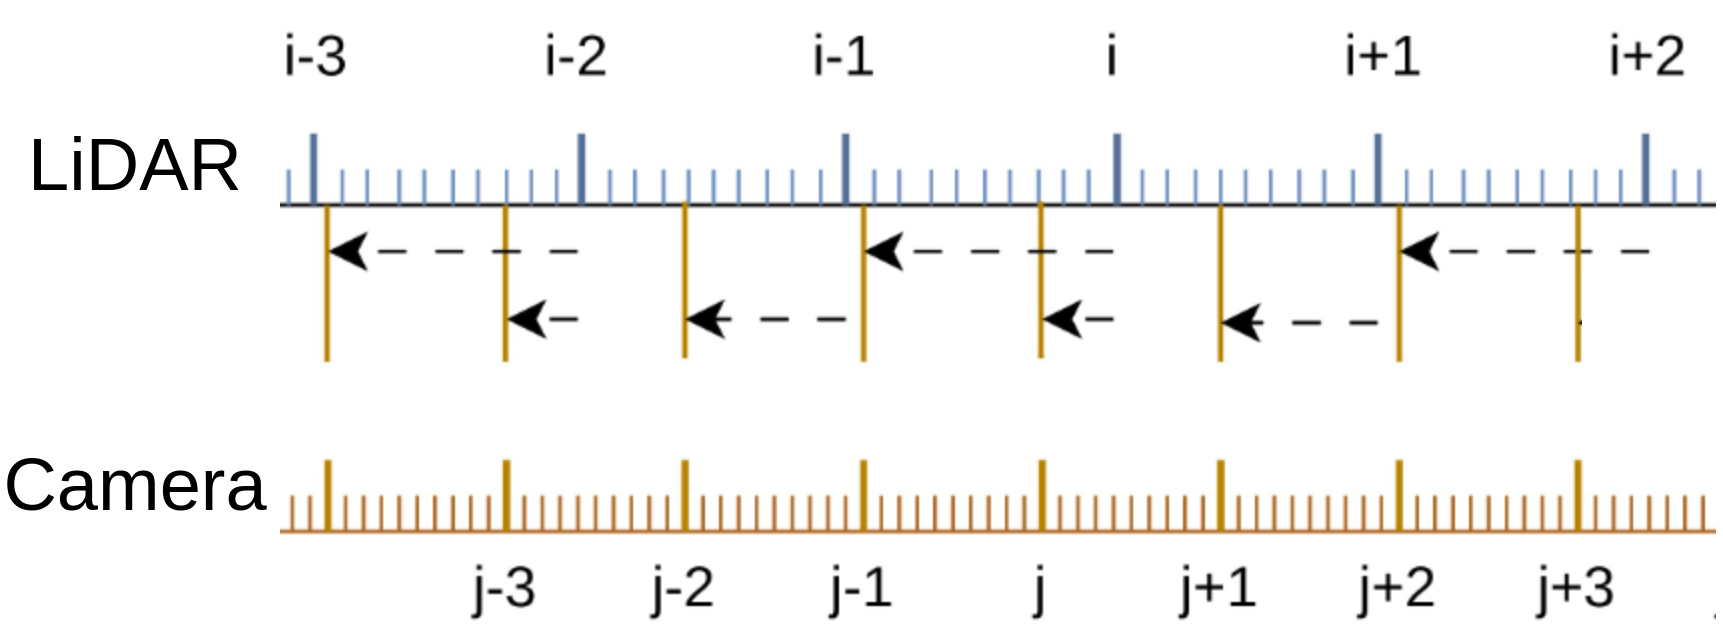
\includegraphics[width=0.42\textwidth]{images/timestamp_m.png}
  \caption{LiDAR sensor data is aligned to the camera timestamp for temporal consistency.}
  \label{fig:timestamp}
  \vskip -3ex
\end{figure}

After receiving sensor data, each subsystem proceeds to extract geometric features. The visual system utilizes ORB~\cite{rublee2011orb} and LSD~\cite{engel2014lsd} algorithms to detect points and lines in images. On the other hand, the LiDAR system employs PCA algorithm~\cite{hackel2016fast, weinmann2013feature} to extract point, linear, and planar features. To overcome the limitations imposed by individual sensor types, the fusion framework 
%
combines the geometric features and projects them into spherical coordinates, creating a unified representation that incorporates both temporal and spatial dimensions. By performing a K-D tree search, we establish a definitive correlation between the detected lines and the depths of geometric features in the point cloud. This correlation allows us to reconstruct depth measurements for line segments that cannot be accurately triangulated by the visual subsystem alone.

Once reconstructed by the fusion framework, the lines serve as new features with precise depth and are fed back to the subsystems for motion estimation and optimization. In the LiDAR subsystem, the linear directions along the same line can be inconsistent due to sparse point clouds. 
%
The fusion framework determines their average direction, which is used to adjust the directions of the linear features in the LiDAR subsystem, reducing the occurrence of outliers. When both the fusion framework's data association and the visual subsystem's triangulation provide the direction of the same line segment, the visual subsystem introduces a new optimization term called the ``line direction residual''. This term evaluates the angular difference between the two directions. By iteratively minimizing this residual, the system effectively constrains the direction of the line landmarks.

Our system relies on the visual subsystem's output to determine its odometry, which exhibits higher precision in scenes with abundant texture. However, given the increased likelihood of visual SLAM tracking failure, we incorporate a detection module to verify the proper functioning of the visual subsystem. In cases where the visual module fails, the system seamlessly switches to the more reliable LiDAR subsystem to perform pose estimation. This crucial capability ensures enhanced robustness, enabling the system to maintain accurate localization and mapping even in challenging scenarios.

\subsection{Fusion Framework}
\noindent\textbf{Preprocessing - temporal and spatial alignment.} The integration of sparse geometric features from sensors with varying positions and frequencies inherently poses challenges within the unaligned fusion framework. We employ data accumulation and temporal and spatial consistency, enhancing the reliability of our approach effectively.

By accumulating multi-frame point clouds, our system achieves a higher level of detail in the point cloud, comparable to that of the camera image.  This increased resolution allows easier matching of geometric features between the point cloud and the camera image.

Figure \ref{fig:ground_robot} demonstrates that the camera and LiDAR sensors are mounted at different angles and positions. To integrate data from both sensors into a unified coordinate system, we leverage extrinsic calibration. This calibration provides the necessary information about the relative transformation between the camera and LiDAR, enabling accurate alignment of data acquired from both sensors.

To maintain temporal consistency, it is crucial to synchronize data between LiDAR and the camera. We define the camera coordinate system and timestamp as the reference. As illustrated in Figure~\ref{fig:timestamp}, we align the LiDAR point cloud within the time interval from frame $j$ to $j+1$ to the timestamp $t_{j+1}$. During each sweep, we calculate the time difference from each point to the end of the sweep period $t_{j+1}$. Assuming a constant angular and linear velocity over this short period and that the initial pose remains the same as the previous frame, we employ linear interpolation to compute the relative pose for each point and project it onto the timestamp $t_{j+1}$. This process achieves temporal consistency within our system.

\noindent\textbf{Depth and direction association of geometric features.} After achieving spatial and temporal alignment, the geometric features from both subsystems are projected onto a spherical coordinate system centered at the camera. This projection is illustrated in Figure~\ref{fig:arc}, where a 2D visual line segment is projected onto the sphere as an arc. To perform the subsequent neighborhood search, we need to discretize the arcs and ensure a consistent density. To achieve this, we uniformly sample the arc at regular intervals $\Delta \varphi$ by incrementing the angle and determining the corresponding positions of the sampled points.
This sampling process results in a set of points along the arc with uniform spacing.
To process the LiDAR information, we first project the dense geometric point cloud onto a sphere. We then store all LiDAR geometric feature points in a 3D KD-tree~\cite{mark2008computational} and search for the closest geometric neighbor of each point along the visual arc. This iterative process continues until all points along the arc are successfully matched with their corresponding LiDAR feature points. This robust relationship between the visual arc and the LiDAR feature points allows for accurate line reconstruction. 

In the visual frame, we utilize the Line Segment Detector (LSD) algorithm to detect line features by identifying pixel regions with significant gradient changes. The first type comprises lines present on smooth surfaces, \textit{e.g.}, door or window frames. These features are extracted as planar features within the LiDAR point cloud. The second type encompasses linear features, including boundaries between different surfaces or well-defined linear elements, \textit{e.g.}, wall-floor boundaries, or trees. These characteristics are identified as linear features within the LiDAR point cloud.

\begin{figure}
  \centering
  \begin{subfigure}{0.47\linewidth}
    \centering
    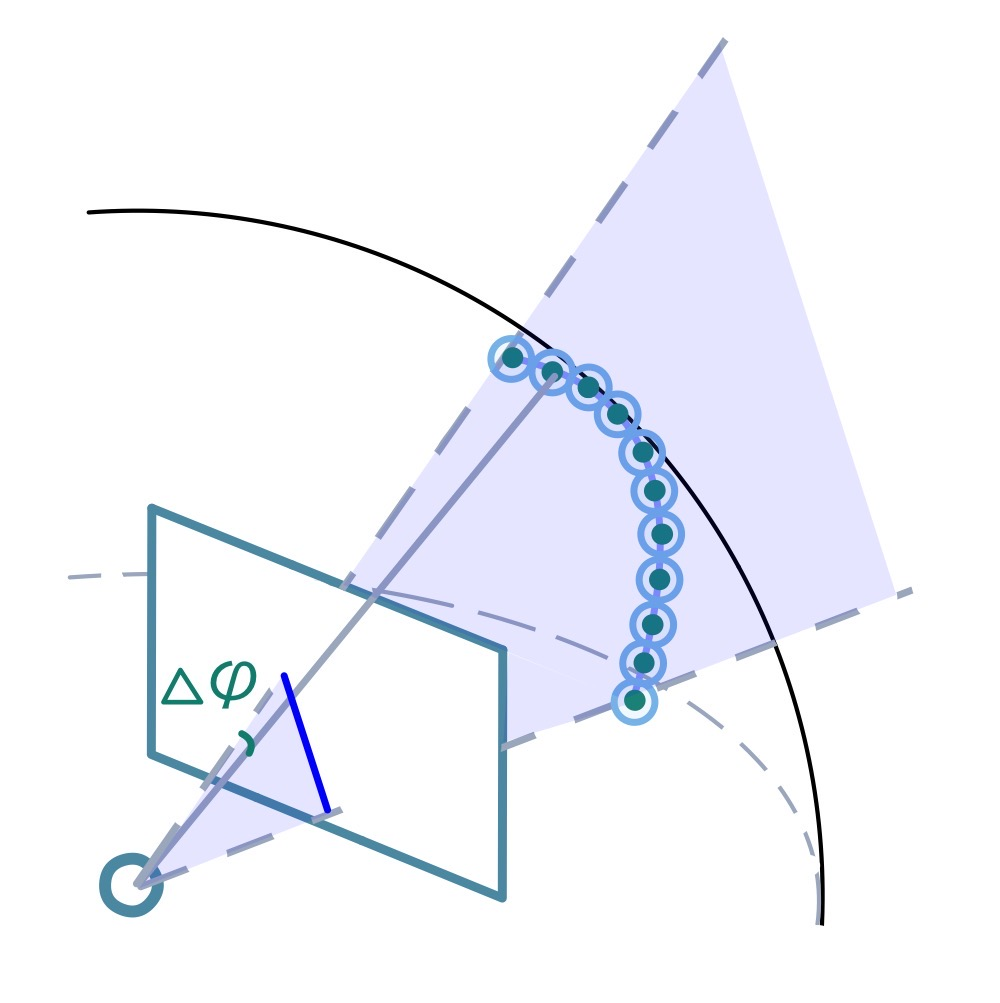
\includegraphics[width=\linewidth]{images/arc_sphere.jpg}
    \caption{Decomposition of the arc into points}
    \label{fig:arc}
  \end{subfigure}
  \hfill
  \begin{subfigure}{0.47\linewidth}
    \centering
    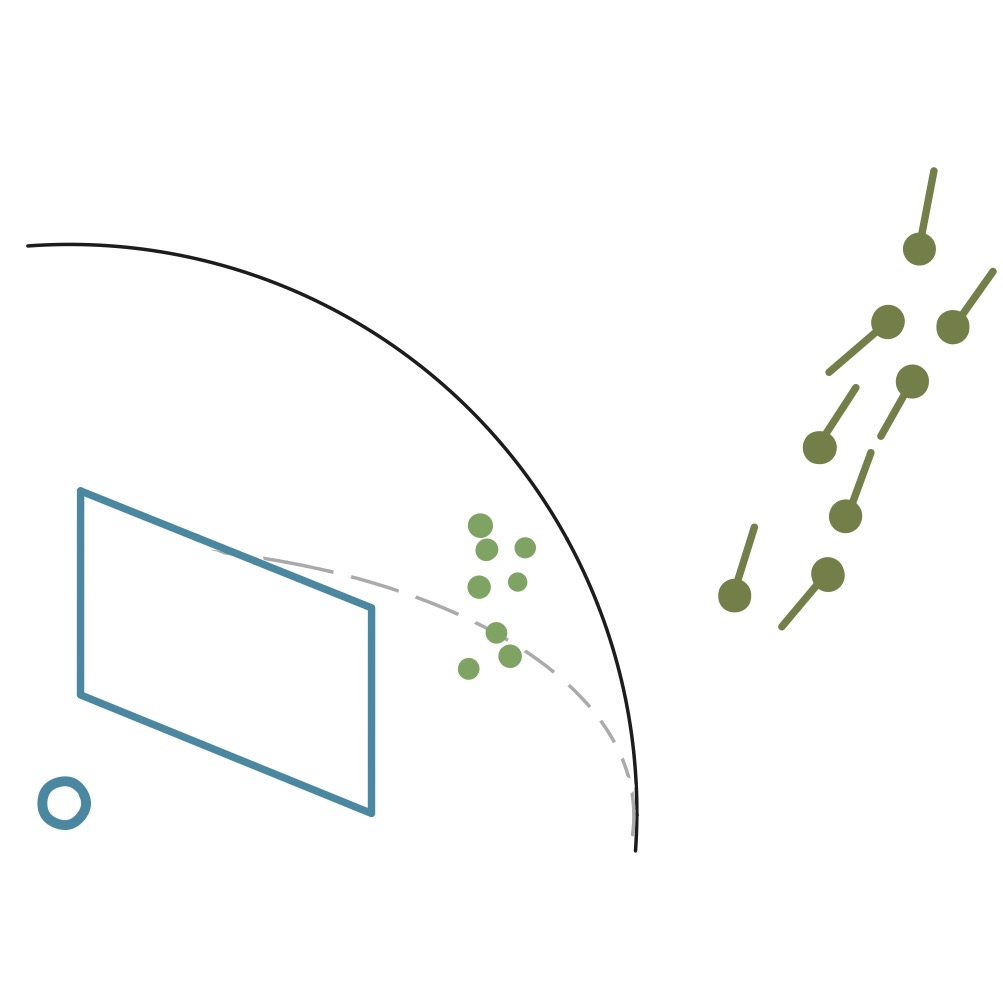
\includegraphics[width=\linewidth]{images/lidar_bad_direction.jpg}
    \caption{Direction of LiDAR linear points before optimization}
    \label{fig:lidar_bad_direction}
  \end{subfigure}

  \vskip -3ex

  \begin{subfigure}{0.47\linewidth}
    \centering
    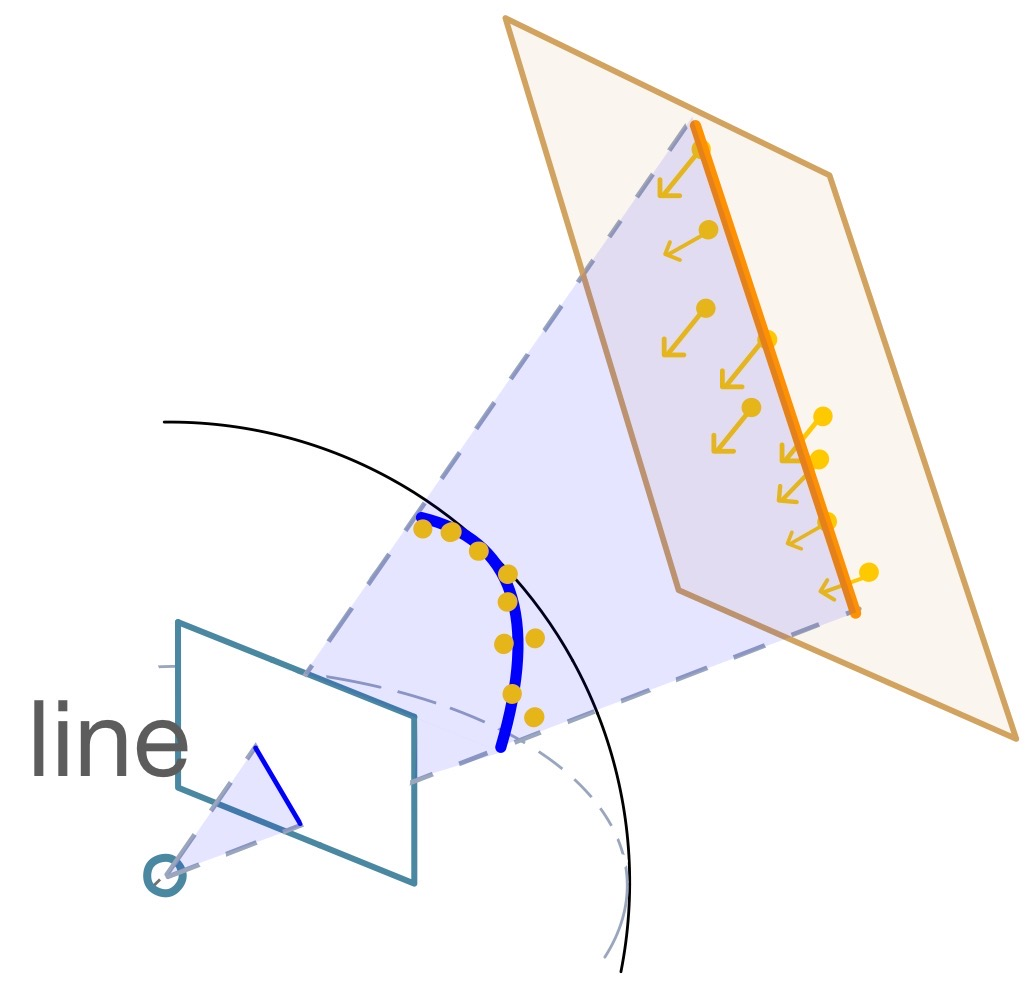
\includegraphics[width=\linewidth]{images/fusion_surface.jpg}
    \caption{Reconstruction line based on LiDAR planar features}
    \label{fig:linear_reconst}
  \end{subfigure}
  \hfill
  \begin{subfigure}{0.47\linewidth}
    \centering
    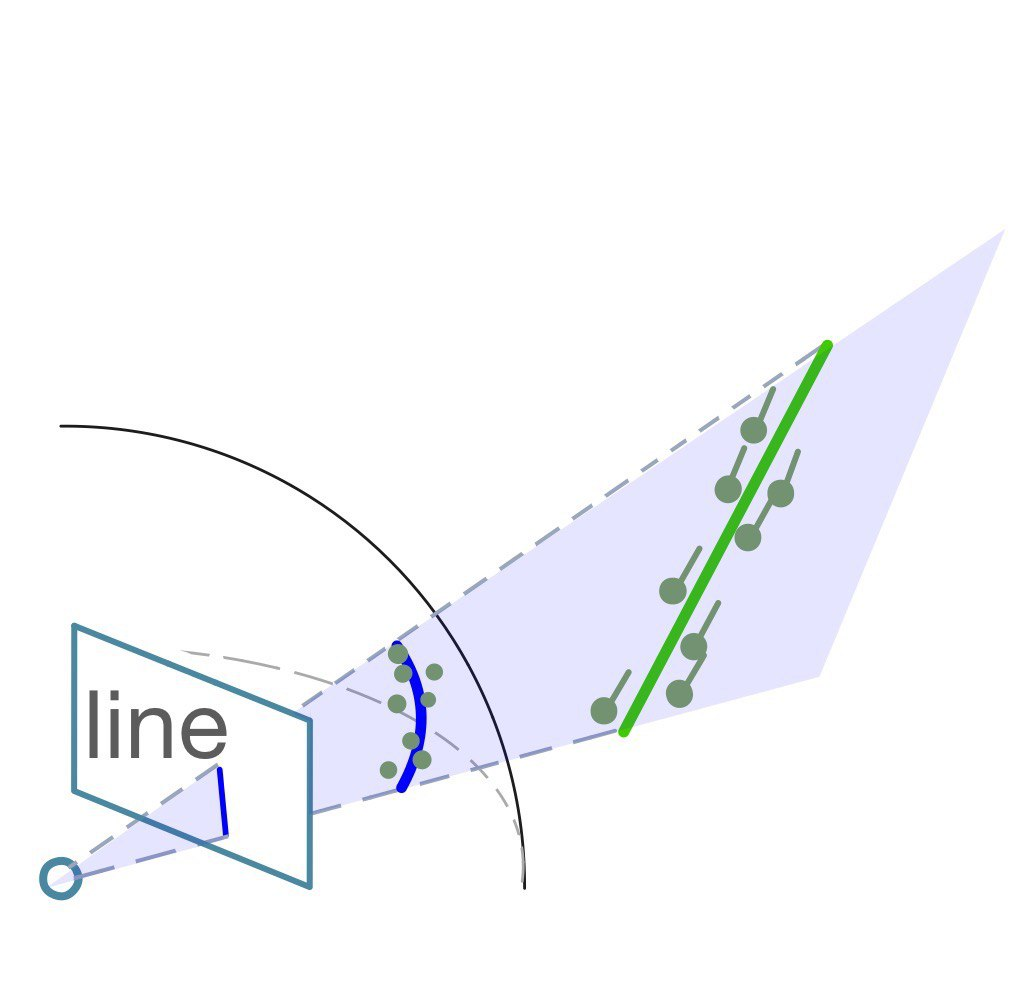
\includegraphics[width=\linewidth]{images/fusion_linear.jpeg}
    \caption{Reconstruction line based on LiDAR linear features}
    \label{fig:planar_reconst}
  \end{subfigure}

  \caption{Processing in the fusion framework.}
  \label{fig:four_images}
  \vskip -3ex
\end{figure}

Therefore, we divide the reconstruction lines, \textit{i.e.}, fusion lines, into two cases. When the majority of the surrounding point cloud comprises planar features, we utilize a plane-to-plane intersection approach to determine the fusion line, as depicted in Figure~\ref{fig:linear_reconst}. Firstly, we reconstruct a virtual LiDAR surface by utilizing appropriate planar feature points and their normal vectors. Subsequently, we project the arc into three-dimensional space, obtaining a projected plane. This plane is then intersected with the LiDAR plane to construct the fusion line.

Alternatively, if the visual arc, as illustrated in Figure~\ref{fig:planar_reconst}, is surrounded by multiple linear features, the points $L_s$ are considered as part of a single line. We select clusters that exhibit similar directions to compute the average line direction, denoted as $L_{best}$. With a point and direction on a line, we determine the line segment based on these linear points.

The fusion frame establishes a spherical coordination system to effectively integrate features from multiple modalities. Under spatiotemporal consistency, the fusion process generates additional lines that are then fed back to the respective subsystems for more accurate localization and mapping.

\subsection{Visual Subsystem}
Our visual subsystem, a derivative of Structure PLP~\cite{shu2022structure}, performs visual SLAM by tracking feature points and feature lines. It comprises three distinct modules, \textit{i.e.}, the line extraction, the line reconstruction, and the joint optimization. Each module leverages information from the visual subsystem and fusion framework to modify and filter out inaccurate data, and assist in pose optimization. 
%

\noindent\textbf{Line detection.} During the feature extraction, we utilize the LSD~\cite{engel2014lsd} algorithm to detect line segments. To enhance the performance of LSD, we refine hidden parameters and implement length rejection, following the methodology of Structure PLP~\cite{shu2022structure}. These modifications contribute to improving the computational efficiency and accuracy of our visual system during feature extraction.

\noindent\textbf{Line reconstruction with triangulation} To reconstruct the detected lines in 3D space, we utilize two methods. The first method involves triangulating the matched line segments across two frames. By using the observed endpoints ${x_s, x_e}$ of a line segment $z$, we calculate the line vector ${l} = {x}_s \times {x}_e$. Using the camera projection matrix $P\in \mathbb{R}^{3 \times 4}$, which only contains the intrinsic camera parameters, we project the observed 2D line onto the camera coordinate system. This projection results in the projection plane $\pi_i = {l}_i^{\top} \mathrm{P}_i$.

The intersection of the two projection planes $\pi_1$ and $\pi_2$ forms a 3D line in world coordinates. We represent this line using the Plücker coordinate system, denoted as $\mathbf{L}=\left(\mathbf{m}^{\top}, \mathbf{d}^{\top}\right)^{\top}$. To obtain its dual Plücker matrix $L^*_w$, the following calculation is performed:
\begin{equation}
\mathrm{L^*_w}=\pi_{1}\pi_{2}^{\mathrm{T}}-\pi_{2}\pi_{1}^{\mathrm{T}}\in\mathbb{R}^{4\times4}
\end{equation}

If the line cannot be successfully triangulated but is provided by the fusion framework, we need to convert this line segment from the Cartesian coordinate system to the Plücker coordinate system. 

Given two endpoints of the 3D lines $\overline{\mathbf{A}}$  and $\overline{\mathbf{B}}$, it is deduced that $\mathbf{L}=\left(\mathbf{m}^{\top}, \mathbf{d}^{\top}\right)^{\top}$ with
\begin{equation}
\left\{\begin{array}{l}
\mathbf{m}=\overline{\mathbf{A}} \times \overline{\mathbf{B}} \\
\mathbf{d}=\overline{\mathbf{B}}-\overline{\mathbf{A}}
\end{array}\right.
\end{equation}

\noindent\textbf{Endpoints trimming.} Line landmarks may have errors due to triangulation using only two frames. Similarly, line reconstruction in fusion frames can suffer from inaccuracies, particularly due to potential imperfections in the spatio-temporal alignment of two-sensor data. Therefore, we refine the endpoints with the method proposed in \cite{lee2019elaborate, zhang2015building}. 

In Structure PLP, endpoint trimming is utilized in local bundle adjustment (LBA). After this trimming, a depth check is performed with a threshold ratio of $0.1$ to filter out outliers based on the median depth change ratio of the scene. Considering the higher confidence in lines from the fusion framework, the outlier rejection threshold is set to $0.2$ for fusion line segments. 
%

\noindent\textbf{Endpoints re-projection and direction residual of line.} Once the observed line segment is detected, we calculate the distances between the endpoints $x_s$ and $x_e$ of the observed line segment $z$ and the projected line segment $l'$. The residual of the line measurement model is defined as the following reprojection error:
\begin{equation}
e_{dis}=d(z,l')=\begin{bmatrix}
\frac{\mathbf x_s^\top \mathbf l'}{\sqrt{l_1^{2}+ l_2^{2}} }   & \frac{\mathbf x_e^\top \mathbf l'}{\sqrt{l_1^{2}+ l_2^{2}} }
\end{bmatrix}^\top
\end{equation}

Many visual SLAM systems that use line features focus primarily on optimizing endpoints while ignoring their directions. Due to the considerable length of fusion line segments, their direction tends to be reliable. We introduce a new type of optimization, called ``line direction optimization'', which imposes additional constraints on the direction of line landmarks.

In our method, we compare the direction $\mathbf d_{fu}$ of the fusion line with the reconstructed line direction $\mathbf d_{cam}$ obtained from the visual subsystem. We unitize the two direction vectors and introduce an additional optimization term to measure the angle between these unit vectors:
\begin{equation}
\begin{aligned}
e_{dir}&=1-\cos (\mathbf d_{cam}, \mathbf d_{fu}) \\
& = 1 -
\frac{\mathbf d_{cam}^\top \mathbf d_{fu}}{\sqrt{d_{cam1}^{2}+ d_{cam2}^{2}} \sqrt{d_{fu1}^{2}+ d_{fu2}^{2}} }
\end{aligned}
\end{equation}

Considering the increasing gradient of this error term with larger errors, we incorporate a robust cost function. This effectively mitigates the influence of outliers, improving the overall stability of the optimization process. 
Moreover, since the angle measurement is independent of the image pyramid level, there is no need to introduce an information matrix.

\begin{figure}
  \centering
  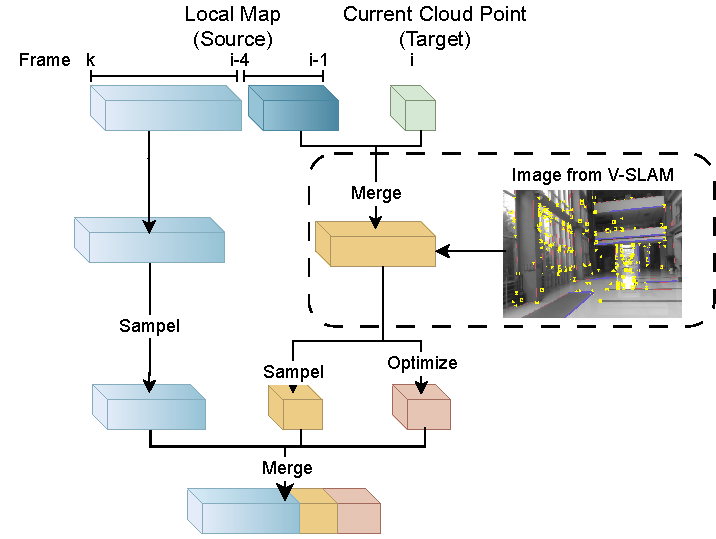
\includegraphics[width=0.5\textwidth]{images/local_map.pdf}
  \caption{An overview regarding the local map update for ICP. The point cloud of the last four frames and the current frame participate in the fusion process with the visual subsystem. The optimized point cloud is kept or sampled less. The unoptimized point clouds are downsampled. Finally, all point clouds are merged to update the local map.}
  \label{fig:local_map}
  \vskip -3ex
\end{figure}

\subsection{LiDAR Subsystem}
Following on the LiDAR SLAM MULLS~\cite{pan2021mulls}, we propose modifications to optimize our LiDAR subsystem. 
%

\noindent\textbf{Modification of the linear direction.} The geometric characteristics of each point are analyzed using the Principal Component Analysis (PCA) algorithm~\cite{hackel2016fast, weinmann2013feature}. PCA determines the local neighborhood of a point and computes the eigenvalues $\lambda_{1} \geq \lambda_{2} \geq \lambda_{3} \geq 0$ and their corresponding eigenvectors $\mathbf{e}_{1}, \mathbf{e}_{2}, \mathbf{e}_{3}$. Following these methods~\cite{hackel2016fast, weinmann2013feature}, we classify points as either linear or planar based on their one-dimensional (1D) linear structure $L_{\lambda}=\frac{\lambda_{1}-\lambda_{2}}{\lambda_{1}}$, two-dimensional (2D) planar structure $P_{\lambda}=\frac{\lambda_{2}-\lambda_{3}}{\lambda_{1}}$, and curvature measurements $C_{\lambda}=\frac{\lambda_{3}}{\lambda_{1}+\lambda_{2}+\lambda_{3}}$. 
%
The geometric features are categorized into five types: vertex, pillar, beam, facade, and roof. 

In the PCA, the size of the local neighborhood is typically limited. This limitation poses challenges in larger scenes where the structural analysis may not be fully exploited. As depicted in Figure~\ref{fig:lidar_bad_direction}, the calculated line directions along the same line exhibit slight variations. These errors have a negative impact on the point-to-line alignment within the Iterative Closest Point (ICP) process. So we leverage detected complete lines in our visual subsystem to gain a more comprehensive understanding of the line structures in the environment. Following the fusion process, we determine which LiDAR linear points ($L_s$) belong to the same line with a consistent line direction. This association allows us to group related linear points together. Then, in the fusion framework, we calculate the mean direction ($\mathbf d_{v\_mean}$) of these lines and update the direction of all linear points by assigning them the calculated mean direction ($\mathbf d_{v\_mean}$).

\noindent\textbf{Improved storage of fusion-enhanced point cloud.} After performing the Iterative Closest Point (ICP) algorithm~\cite{besl1992method}, the target cloud must be updated for the next frame. MULLS merges and downsamples multiple historical frames into the local map. During this process, it is essential to synchronize the point clouds from different timestamps to the current timestamp $i$. This synchronization ensures that the point clouds are correctly aligned and accurately represent the environment. Although the denser local map provides a more comprehensive representation of the environment structure, merging too many historical frames means that the local map has to perform multiple alignments with the estimated pose, which leads to error accumulation. 

In order to strike a balance between preserving important geometric features and minimizing the accumulation of historical frames, a series of steps are employed in our method. As shown in Figure \ref{fig:local_map}, we combine the point cloud from the last four frames with the current frame. These point clouds are then projected onto a sphere to optimize the directions of their linear features. The optimized feature points increase the convergence speed of the ICP and improve the accuracy of the estimated values. Once the point cloud is optimized, we proceed to sample and merge them. To control the density of the local map, we introduce a threshold parameter $\alpha$ that represents the maximum rate of optimized features allowed in the local map. If the current rate of optimized points does not exceed $\alpha$, no sampling is performed. If the rate surpasses the threshold $\alpha$, we downsample the point cloud to reduce the rate until it falls below the specified threshold. Finally, the local map is updated by merging all the point clouds together.